
\documentclass[journal]{IEEEtran}
%\usepackage{lineno}
%\linenumbers
%\usepackage{cite}
\usepackage{comment}
\ifCLASSINFOpdf
  \usepackage[pdftex]{graphicx}
  \graphicspath{pics/}
  \DeclareGraphicsExtensions{.pdf,.jpeg,.png,.jpg}
\else

\fi
\usepackage{amsmath}
\usepackage{siunitx}
\usepackage{geometry}
\usepackage{comment}
\usepackage{float}
\usepackage[caption=false]{subfig}
\usepackage[super]{nth}
\hyphenation{}

\begin{document}
\newgeometry{top=12mm, bottom=12mm, left=12mm, right=12mm}
\title{22051 - Assignment number 1}
\author{\vspace{-2mm}{\normalsize \underline{Group 3} - s194048 Erik Rame ( hrs), s194051 Jakob Bernhardt (14 hrs), s194006 Steffan Kunoy (8 hrs), \\s186083 Tjark Petersen (7 hrs)}\vspace{-10mm}}

% make the title area
\maketitle
%\IEEEpeerreviewmaketitle

\section{Simple filters with poles and zeros}
The objective of this exercise was to gain experience working with the \textit{z}-transform and filters. In particular, the tasks highlighted how the placement of poles and zeros on the unit circle dictated the characteristic frequency response of for example a running-sum or a high-pass filter.
\subsection{The z-transform}
Generally, the \textit{z}-transform of a discrete-time signal $x(n)$ into the complex \textit{z}-plane is given by the \textit{bilateral} forward transform: 
\begin{equation}
\label{eqn:z_transform}
    X(z) = \sum_{n=-\infty}^{\infty} x(n) \cdot z^{-n}
\end{equation}
However, since our signals are assumed to be causal, the \textit{unilateral} transform starting at $n=0$ is used. For instance, the \textit{z}-transform of a \nth{3} order running sum filter $h(n)$, which is simply a summation of 4 terms: 
\begin{equation}
\label{eqn:third_order_rs}
    H(z) = \sum_{n=0}^{\infty} h(n) \cdot z^{-n} = z^{0} + z^{-1} + z^{-2} + z^{-3} 
\end{equation}

\subsection{Poles and zeros}
Using algebraic manipulation, we can express (\ref{eqn:third_order_rs}) as a ratio of polynomials:  
\begin{equation}
\label{eqn:third_order_rs_tf}
    H(z) = \frac{z^3+z^2+z^1+1}{z^3}
\end{equation}
The roots of the denominator and numerator polynomials, known as poles and zeros respectively, dictate the frequency response of an \nth{3} order running sum filter with $H(z)$ as its transfer function. \\
A normalized frequency can be mapped to a point on the unit circle by $z \rightarrow e^{j \omega}$. The magnitude response at this frequency is then given as a ratio of products of the distances to each zero and pole respectively. Thus, as the frequency approaches a zero on the unit circle, a distance in the numerator goes to zero, causing attenuation in the magnitude response at this frequency. Likewise, if the frequency hits a pole, a distance in the denominator becomes zero, causing amplification in the magnitude response at this frequency. \\
\begin{figure}[H]
    \centering
    \captionsetup[subfloat]{farskip=0pt,captionskip=0pt}
    \subfloat[\nth{3} order running sum]{
        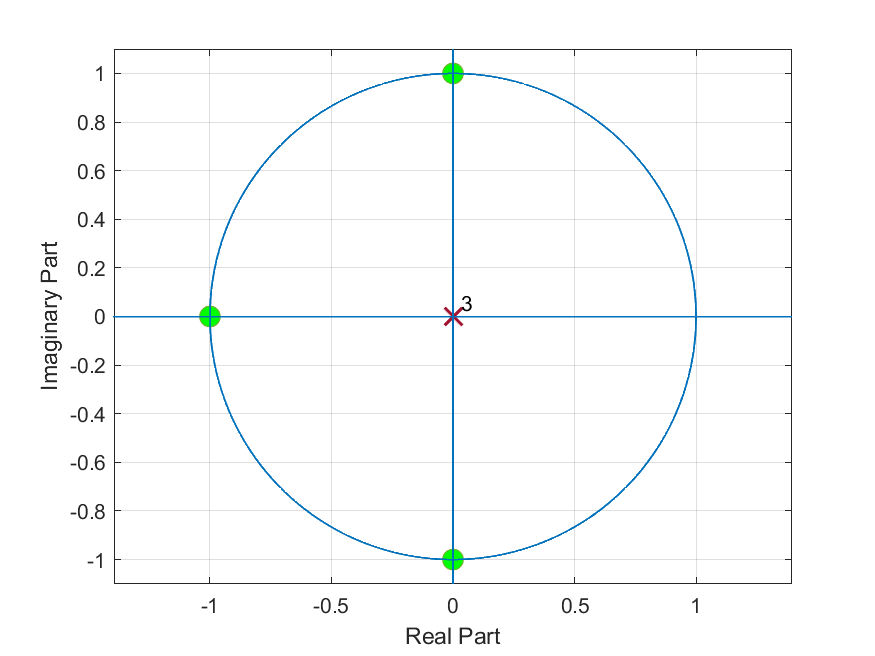
\includegraphics[width=0.5\columnwidth]{assignment_01/plots/3rd_order_running_sum_z_plane.png}
        \label{fig:zplane_a}
    }
    \subfloat[\nth{5} order running sum]{
        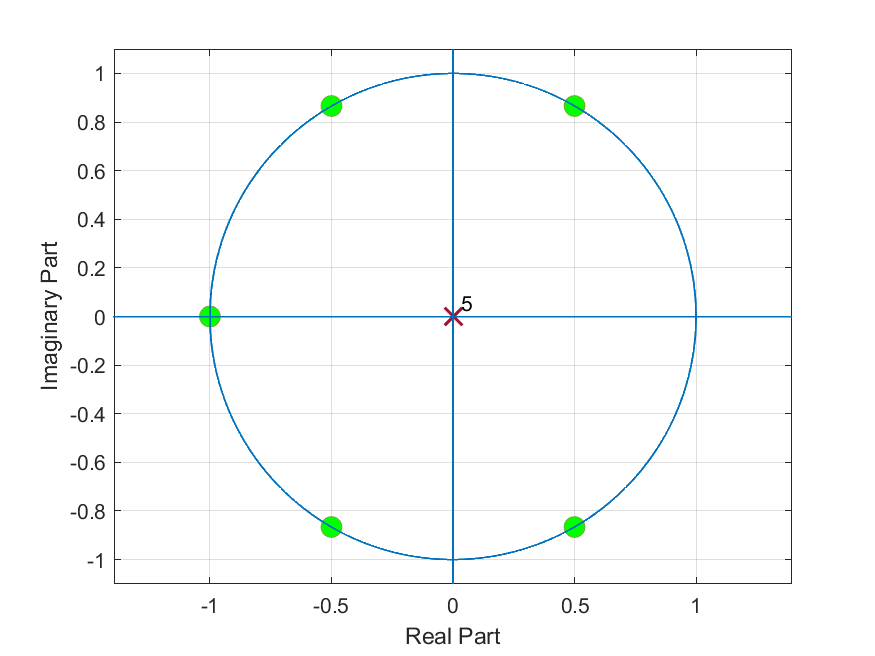
\includegraphics[width=0.5\columnwidth]{assignment_01/plots/5th_order_running_sum_z_plane.png}
        \label{fig:zplane_b}
    }
    \caption{Placement of filter poles and zeros on the complex \textit{z}-plane.}
    \label{fig:zplane}
\end{figure}
We can observe this phenomenon for the poles and zeros of the \nth{3} order running sum filter, which are plotted on the complex \textit{z}-plane in Figure \ref{fig:zplane_a}. Its frequency response, shown in Figure \ref{fig:freq_resp1_a}, is heavily attenuated at the normalized frequencies $\frac{\pi}{2}, \pi \text{ and } \frac{3 \pi}{2}$, corresponding to the arguments of each of its three zeros. The triple pole at the origin does not affect the frequency response as its distance is always constant. Likewise, the frequency response of the \nth{5} order running sum filter in Figure \ref{fig:freq_resp1_b} is also affected by its pole-zero locations shown in Figure \ref{fig:zplane_b}. 
\begin{figure}[H]
    \centering
    \captionsetup[subfloat]{farskip=0pt,captionskip=0pt}
    \subfloat[\nth{3} order running sum]{
        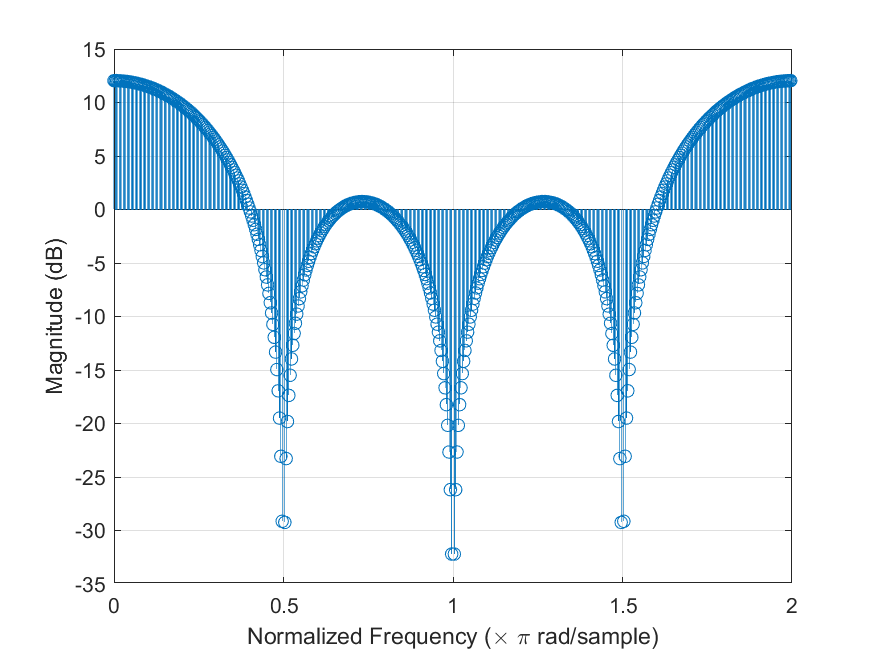
\includegraphics[width=0.5\columnwidth]{assignment_01/plots/3rd_order_running_sum_freq_resp.png}
        \label{fig:freq_resp1_a}
    }
    \subfloat[\nth{5} order running sum]{
        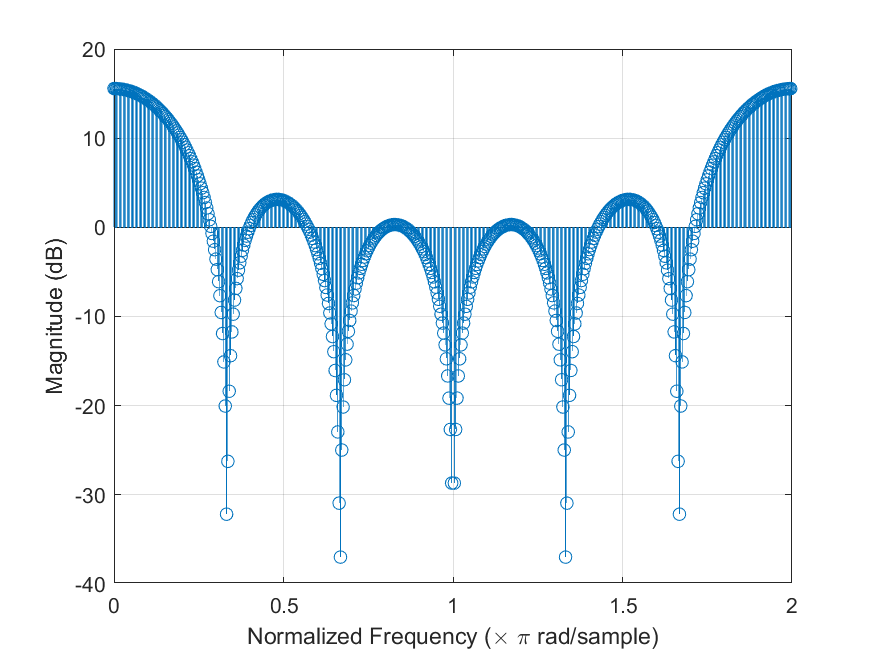
\includegraphics[width=0.5\columnwidth]{assignment_01/plots/5th_order_running_sum_freq_resp.png}
        \label{fig:freq_resp1_b}
    }
    \caption{Filter frequency responses plotted on the normalized-frequency axis.}
    \label{fig:freq_resp1}
\end{figure}

\subsection{Filtering} 
As seen in the previous section, we can control the frequency response of an LTI-system simply by placing its poles and zeros at appropriate locations on the \textit{z}-plane. Placing a single real zero at some distance \textit{r} in the LHP and no poles creates a \textbf{low-pass} filter, while placing a single zero at the same distance in the RHP with no poles yields a \textbf{high-pass} filter. Placing an equal number of poles and zeros at the exact same locations meanwhile produces an \textbf{all-pass} filter. The value of \textit{r} determines the level of attenuation for zeros or amplification for poles, with $r=1$ constituting the maximum and $r=0$ having no effect on magnitude.\\
Passing a signal through these filters requires convolution in the time domain, or simply multiplication in the \textit{z}-domain. Figure \ref{fig:filtered_sound} shows the result of filtering a sound signal sampled at 44.1 kHz with a low-pass, high-pass and all-pass filter. 
\begin{figure}[H]
    \centering
    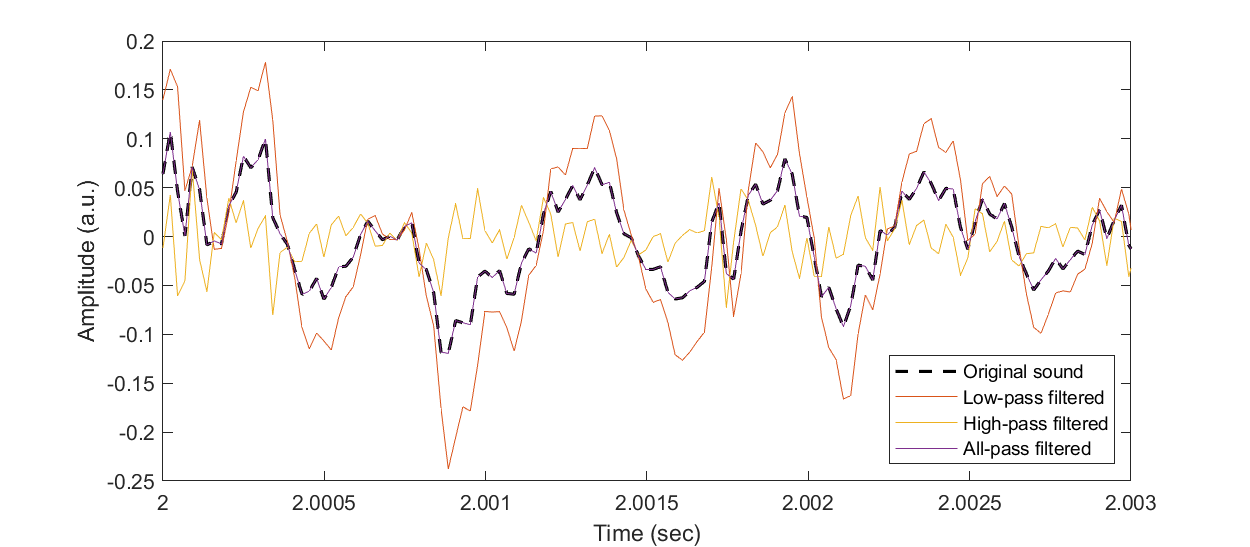
\includegraphics[width=\columnwidth]{assignment_01/plots/filtered_sound.png}
    \caption{Result of passing a sound signal through the different filter types.}
    \label{fig:filtered_sound}
\end{figure}
From this time-domain plot we can see that the low-pass filter amplifies the signal amplitude while the high-pass filter attenuates it. This is due to the high sampling rate which "pushes" the frequency spectrum into the passband of the low-pass filter and the stopband of the high-pass filter. when compared with the frequency spectrum. As expected, the all-pass filter has no effect on the signal amplitude. 
\clearpage

\section{Room model using sound reflections}

In this section two system models for the acoustic behavior of a room are examined. Both models try to capture the reflection of sound waves of the rooms walls. The first model achieves this using a single reflection after a certain delay, resulting in an FIR filter. The other model uses feedback to create a never ending series of increasingly attenuated reflections, resulting in an IIR filter.

The FIR filter is described by the difference equation:
\begin{equation}
    y(n) = x(n) + \alpha x(n-delay)
\end{equation}

This can be transformed to the $z$-domain resulting in:
 \begin{equation}
     Y(z) = X(z) + \alpha X(z) z^{-delay}
 \end{equation}
 \begin{equation}
     H_{FIR}(z) = \frac{z^{delay} + \alpha}{z^{delay}}
\end{equation}

The IIR filter on the other hand is described by the difference equation:
\begin{equation}
    y(n) + \alpha y(n-delay) = x(n)
\end{equation}

The $z$-domain transfer function can be determined to be:
\begin{equation}
    Y(z) + \alpha Y(z) z^{-delay} = X(z)
\end{equation}
\begin{equation}
    H_{IIR}(z) = \frac{z^{delay}}{z^{delay} + \alpha}
\end{equation}

We can see that the transfer functions of the two models are actually the inverse of each other. The FIR filter has $delay$ zeros spread evenly around the unit circle and a pole at the origin with a multiplicity of $delay$ and vice versa for the IIR model.

The inverse nature of the two models also becomes apparent in their spectra. Figure \ref{fig:bounce:spectra} shows a small section of the very densely packed spectra of the FIR and IIR implementations using a time delay of $\SI{30}{ms}$, resulting, at a sampling frequency of $\SI{44.1}{kHz}$, in a delay of 1323 samples. Both use a value of 0.6 for $\alpha$. It can be observed that the spectra are periodic and when studying the spectra with different time delays, that the period is determined by the time delay of the implementation.

When studying the impulse responses (see figure \ref{fig:bounce:impulse}) the similarities between the two models vanish but we can see the expected behavior: The FIR filter repeats the input signal slightly attenuated once after a certain number of samples whereas the IIR reflects an increasingly attenuated version of the input signal indefinitely. Longer delays result in the reflections occurring later in time.

The effect of the two filter models on a signal can be studied in figure \ref{fig:bounce:signals}. The reflected versions of the signal add to the original signal and make it harder to identify. This translates to the original signal being harder to hear when listening to the filtered version. The longer the time delay, the larger the number of different reflections that add to the original signal in a small time interval and the original signal gets even less identifiable. Since the IIR filter produces a never ending series of reflection, it creates signals where the original signal is hardest to identify.

Listening to both filters, the IIR based filter clearly sounds more realistic and thus seems to be the superior model.

\begin{figure}
    \centering
    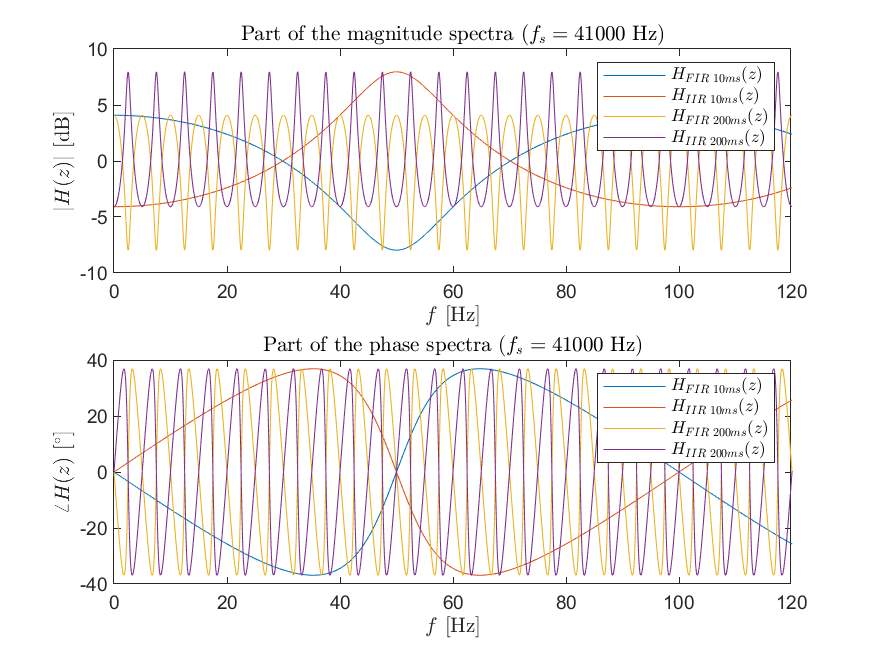
\includegraphics[width=\linewidth]{assignment_01/plots/bounce_spectra.png}
    \caption{Part of the spectra for both room models with a time delay of $\SI{30}{ms}$.}
    \label{fig:bounce:spectra}
\end{figure}
\begin{figure}
    \centering
    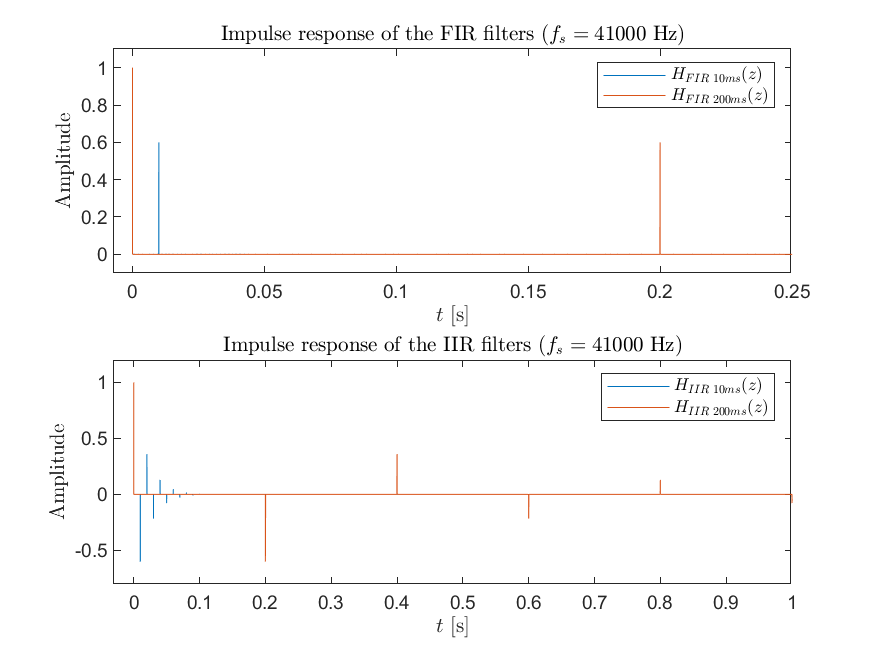
\includegraphics[width=\linewidth]{assignment_01/plots/bonuce_impulse.png}
    \caption{Impulse responses for both room models with a time delay of $\SI{30}{ms}$.}
    \label{fig:bounce:impulse}
\end{figure}
\begin{figure}
    \centering
    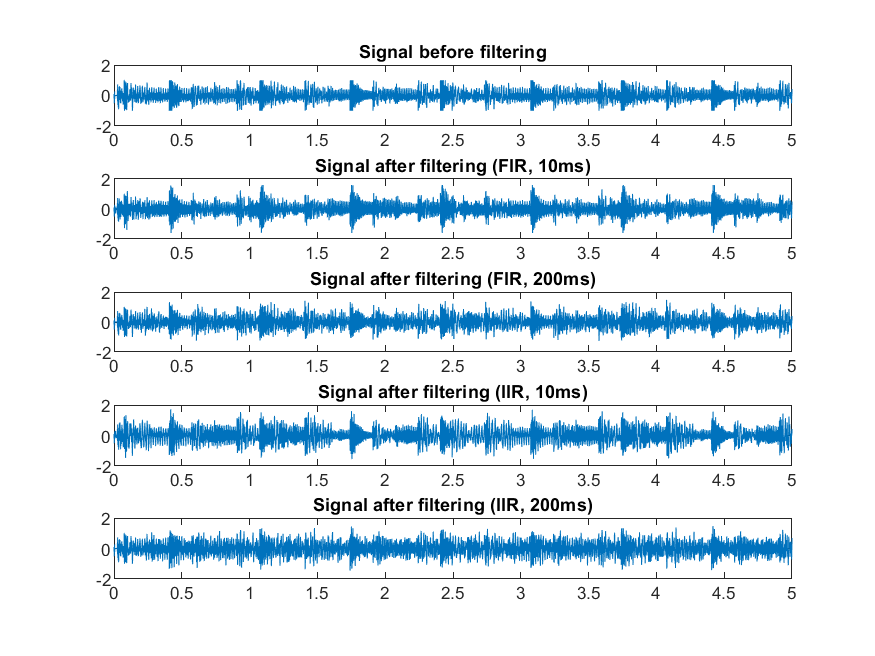
\includegraphics[width=\linewidth]{assignment_01/plots/bounce_signals.png}
    \caption{Application of the two models on a signal with a time delay of $\SI{30}{ms}$.}
    \label{fig:bounce:signals}
\end{figure}

\newpage
\section{Signal Generation and Data Saving (Hands-On 1)}
Knowing that we would be generating discrete sinusoids, the according parameters first had to be declared and defined, those being the sampling frequency, duration of time we choose to investigate, sampling frequency and, of course, the number of components to each signal we wish to implement. The way the code was designed, it starts by defining three vectors, one of which contains all 0's, another with all $\pi/2$'s and one with random numbers in the interval 0 to $2\pi$. These represent the phase angles used in the different signal summations. The code then initiates a for loop that cycles through each each element of the phase vectors generating a sinusoid of the form given in the exercise, whilst using the corresponding phase angle and adding it to the existing summed sinusoids. Once all the elements had been run through, it would create a .wav file for each of the summed phase sinusoids. They are then plotted and the plots are saved as .png files. Below that another graph showing all three graphs plotted together with a smaller x-axis are shown, to make it easier to assess the effect of N on the graphs. Playback is possible by uncommenting the central code block and running it. Below are the graphs generated by setting the sinusoids to be sums(N) of 3 (condensed here to show all 3 on one figure):
\newline
\begin{figure}[H]
    \centering
    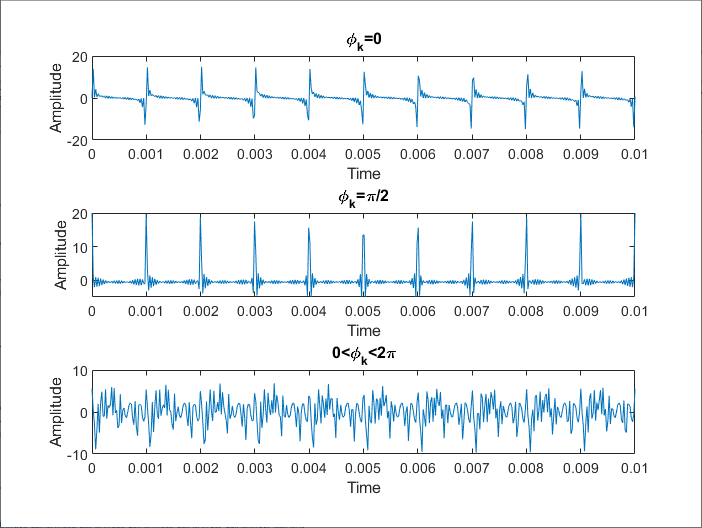
\includegraphics[width=\linewidth]{assignment_01/plots/PHs.png}
    \label{fig:zeroph}
\end{figure}

\textbf{\textit{Is there some limit of N that needs to be considered here?}}
\newline
As we know we have audio signals with a sampling rate of 44.1 kHz, it would be unwise to use an N of higher than half of the sampling frequency, as this would result in aliasing. Since our fundamental frequency is 1kHz, and as we generate a new harmonically related frequency signal with each higher N, an N of no more than 22 should be used to guarantee complete signal reconstruction.
\newline
\begin{equation}
     f_N < 2 \cdot f_s
\end{equation}
\newline
The effect of altering the number of harmonically related sinusoids can be seen in the next column, where an N of 3, 10 and 20 have been used;
\newline
\begin{figure}[H]
    \centering
    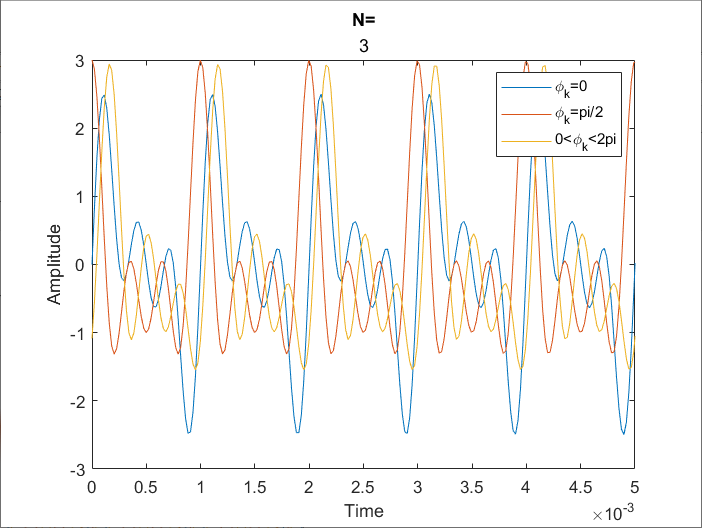
\includegraphics[width=9cm]{assignment_01/plots/N=3.png}
    \label{fig:N=3}
\end{figure}

\begin{figure}[H]
    \centering
    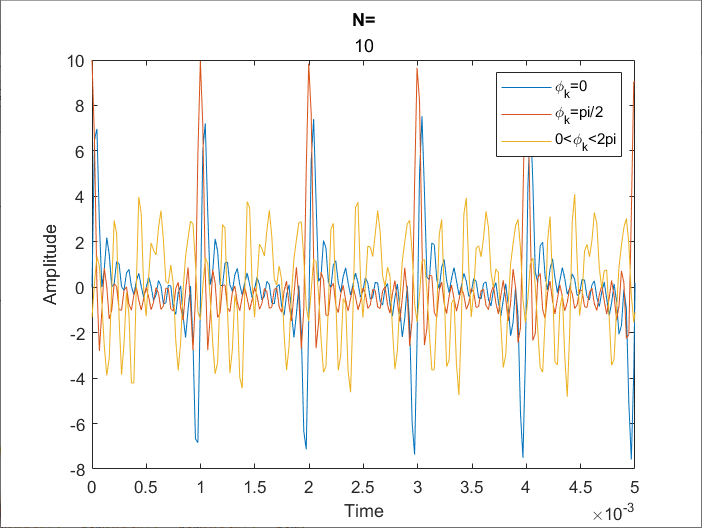
\includegraphics[width=9cm]{assignment_01/plots/N=10.png}
    \label{fig:N=10}
\end{figure}

\begin{figure}[H]
    \centering
    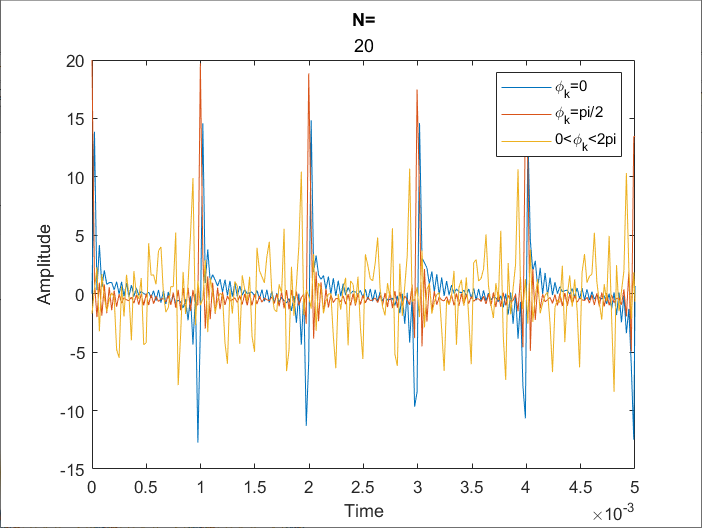
\includegraphics[width=9cm]{assignment_01/plots/N=20.png}
    \label{fig:N=20}
\end{figure}

Whilst changing the number of summed sinusoids of course increases the frequency and amplitude of the apparent sound, the difference between the phased signals is somewhat harder to identify. Those in phase sound clearer, almost sharper than those whose phase is random, which sound noisier and rather unclear (blown out speaker?).

\section{Fourier transform of a recorded signal (Hands-on 3)}
% first have a section with a short explanation of fourier transform mathematically, then go into the details of the exercise and what the following sections describe/show/include and also the results 
To analyze the composition of a recorded signal, it is often more practical to examine it in the frequency domain. To move from the time-domain into the frequency domain, we use Fourier transform. 
Hands-on 3 exercise 1.3 dealt with the Fourier transform of a recorded signal. The sound sample of a piano playing a single note 'piano.wav' was loaded into MATLAB. The discrete time signal 'piano.wav' is made up of many frequency components, and the Fourier transformation is a sort of decomposition of the signal into its frequencies. As a result, we can see how much of each frequency is contained within the signal.

\subsection{Signal plots and Fourier analysis}
% describe the methods used, and explain why you choose your specific approach! restrict yourself to the most essential information. provide all information necessary to reproduce your results
In order to learn about the composition of the sound signal, the signal was plotted in the time and frequency domain (see figure \ref{fig:time} and \ref{fig:freq}). 

\begin{figure} [h]
    \centering
    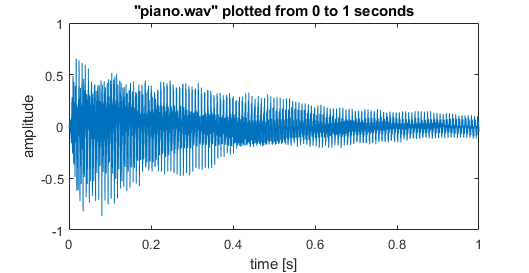
\includegraphics[width=\linewidth]{assignment_01/plots/time_plot.png}
    \caption{Recorded signal plotted in the time-domain from 0 to 1 s.}
    \label{fig:time}
\end{figure}
\begin{figure} [h]
    \centering
    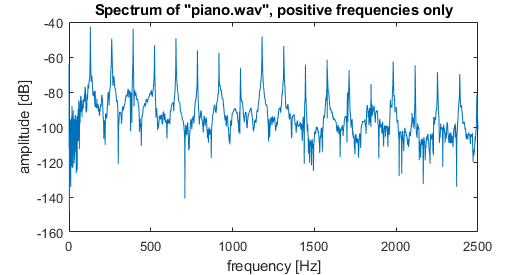
\includegraphics[width=\linewidth]{assignment_01/plots/freq_plot.png}
    \caption{Power spectrum of recorded signal. Only positive frequencies, including the DC component, are shown; specifically 0 to 2500 Hz.}
    \label{fig:freq}
\end{figure}

We use discrete Fourier transform to get the spectrum of the whole signal in MATLAB. It is important to note, that MATLABs fft function returns the positive values of the signal spectrum first. The spectrum of the whole signal is plotted with \textit{Hz} and \textit{dB} on the x- and y-axis respectively. % should we show this plot?
To plot only the positive frequencies, including the DC component, we create new frequency and signal vectors, only containing values for the positive frequencies. The resulting plot is shown in figure \ref{fig:freq}.
\newline
From the spectrum in figure \ref{fig:freq}, we can estimate the fundamental frequency of the signal by looking at the spectral peaks. The fundamental frequency is defined as the lowest frequency of a periodic waveform. % wikipedia
We see that the lowest peak is found at 130.43 Hz and therefore, with a precision of 0.5 Hz, we estimate the fundamental frequency of the signal to be
\begin{equation}
    f_0 = 130.5 Hz.
\end{equation}

The fundamental frequency is what we perceive as the musical pitch of a tone. 130.5 Hz roughly correlates with the fundamental of C3 on a piano, which sounds very similar to the tone played in 'piano.wav'. The other peaks in the spectrum represent the harmonics of the tone. 

\subsection{Synthesis}
Using the known distribution of harmonics we got from the Fourier analysis, we can synthesize the sound of the piano. We start out by simply synthesizing the signal for 2 seconds in the frequency domain by approximating it with a harmonic series. Here, we add sine waves of varying frequencies and amplitudes together to get the desired timbre of our synthesized signal. 
\begin{figure} [h]
    \centering
    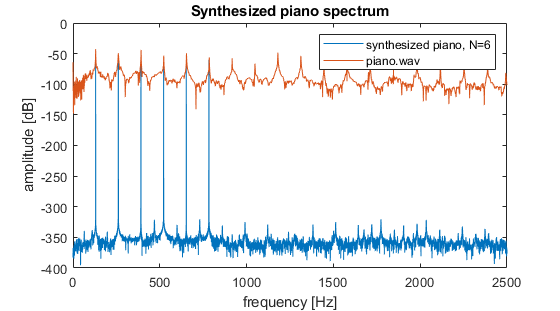
\includegraphics[width=\linewidth]{assignment_01/plots/synth.png}
    \caption{A spectrum comparison of 'piano.wav' and a synthesized piano.}
    \label{fig:synth}
\end{figure}
\newline
Figure \ref{fig:synth} shows a comparison of the power spectrum of the real signal and the synthesized signal. We see that the peaks of the signals match with respect to frequency and magnitude. However, we chose to only use 6 components, and thus the signal lacks detail in the higher components and doesn't sound realistic when we listen to it.
The second part of the synthesis exercise deals with the same components as in the preceding example, but now we also consider phase in addition to magnitude. Although the power spectrums (figure \ref{fig:synth2}) look quite similar, the phases still seem to have an effect on the sound of the synthesized signal.
\newline
\begin{figure} [H]
    \centering
    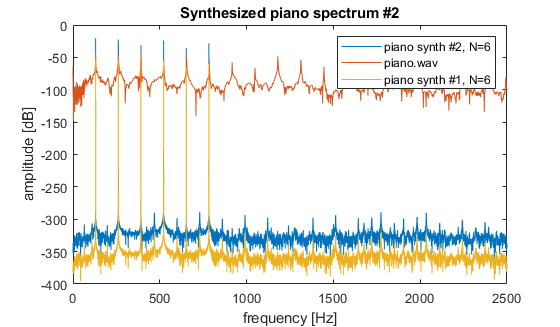
\includegraphics[width=\linewidth]{assignment_01/plots/synth2.png}
    \caption{A spectrum comparison of 'piano.wav', the first piano synth and the second piano synth.}
    \label{fig:synth2}
\end{figure}

% jeg tivler på at den sidste halvdel af synthesis (plot 10) er korrekt

\end{document}


